\documentclass[fleqn,usenatbib]{mnras}

\usepackage{newtxtext,newtxmath}
\usepackage[T1]{fontenc}
\usepackage{ae,aecompl}
%\usepackage{txfonts}
\usepackage{times}

\usepackage{rotating,graphicx}	% Including figure files
\usepackage{amsmath}	% Advanced maths commands
%\usepackage{amssymb}	% Extra maths symbols
\usepackage{ulem}
\usepackage[ampersand]{easylist}

\usepackage{latexsym}
\usepackage{enumerate}% http://ctan.org/pkg/enumerate
\usepackage{amstext}
\usepackage{morefloats}

\usepackage{natbib}
\usepackage{rotating}
\usepackage{changepage}% http://ctan.org/pkg/changepage
\usepackage{scrextend}
\usepackage[ampersand]{easylist}
\usepackage{xcolor}
\usepackage{ulem}

\newcommand{\rt}[1]{{\textcolor{red}{{#1}}}}
\newcommand{\bt}[1]{{\textcolor{blue}{{#1}}}}
\newcommand{\rtc}[1]{{\textcolor{red}{({#1})}}}
\newcommand{\gt}[1]{{\textcolor{}{{#1}}}}
\newcommand{\gtb}[1]{{\textcolor{olive}{[{#1}]}}}
\newcommand{\err}[1]{{\textcolor{cyan}{[{ERR: #1}]}}}
\usepackage{mathtools}
%\usepackage{hyperref}

 
\title[Star Cluster Stellar Wind Retention \& Expulsion]{Should I Stay or Should I Go:  Stellar Wind Retention and Expulsion in Massive Star Clusters}


\author[J.~P.~Naiman et al.]{J.~P.~Naiman$^{1}$\thanks{E-mail: jill.naiman@cfa.harvard.edu}, E.~Ramirez-Ruiz$^{2}$, D.~N.~C.~Lin$^{2}$ 
\vspace*{0.2cm} \\
% List of institutions
$^{1}$Harvard-Smithsonian Center for Astrophysics, 60 Garden Street, Cambridge, MA, 02138, USA\\
  $^2$Department of Astronomy and Astrophysics, University of California, Santa Cruz, CA 95064, USA
}

\date{11 July 2017}

% Enter the current year, for the copyright statements etc.
\pubyear{2017}

% Don't change these lines
\begin{document}
\label{firstpage}
\pagerange{\pageref{firstpage}--\pageref{lastpage}}
\maketitle



\begin{abstract}
Mass and energy injection throughout the lifetime of a star cluster contributes to the gas reservoir available for subsequent episodes of star formation and the feedback energy budget responsible for ejecting material from the cluster.
In addition, mass processed in stellar interiors and ejected as winds has the potential to augment the abundance ratios of currently forming stars, or stars which form at a later time from a retained gas reservoir.
Here we present hydrodynamical simulations that explore a wide range of cluster masses, compactnesses, metallicities and stellar population age combinations in order to determine the range of parameter space conducive to stellar wind retention or wind powered gas expulsion in star clusters.
We discuss the effects of the stellar wind prescription on retention and expulsion effectiveness, using MESA stellar evolutionary models as a test bed for exploring how the amounts of wind retention/expulsion depend upon the amount of mixing between the winds from stars of different masses and ages.
We conclude by summarizing some implications for gas retention and expulsion in a variety of compact ($\sigma_v \gtrsim 20 \, {\rm km s^{-1}}$) star clusters including young massive star clusters ($10^5 \lesssim M/M_\odot \lesssim 10^7$, $age \lesssim 500$~Myrs), intermediate age clusters ($10^5 \lesssim M/M_\odot \lesssim 10^7$, $age \approx 1-4$~Gyrs), and globular clusters ($10^5 \lesssim M/M_\odot \lesssim 10^7$, $age \gtrsim 10$~Gyrs).
\end{abstract}

% Select between one and six entries from the list of approved keywords.
% Don't make up new ones.
\begin{keywords}
galaxies: star clusters: general -- stars: mass-loss -- (Galaxy:) globular clusters: general\end{keywords}

%%%%%%%%%%%%%%%%%%%%%%%%%%%%%%%%%%%%%%%%%%%%%%%%%%



\section{Introduction}
 

 Whether and when gas is retained within a star cluster, along with inter-cluster and intra-cluster gas heating mechanisms determines the star formation history of the cluster.
 Many cluster properties can be responsible for gas retention or expulsion in a cluster - the cluster's compactness, cluster mass, ability to cool effectively, mass and temperature of gas reservoir, and efficiency of internal and external heating mechanisms.  
 As it thought that most stars form in clusters \citep[e.g.][]{lada2003}, the study of which parameters and mechanisms are important at different cluster evolutionary times is crucial to understand when favorable conditions for star formation arise throughout a cluster's lifetime.

 Observations of young massive clusters (YMCs), intermediate age clusters (IACs) and globular clusters (GCs) potentially give us insights into gas retention at different times within massive star clusters \citep[e.g.][]{bastian2017}.
 Additionally, if GCs evolve from YMCs and IACs as some have suggested \citep{longmore2014,krui2015} then observations of each type of system provides clues to the origin of the high level of occurrence of multiple subpopulations with different abundance ratios within present day GCs.

 Variations in the abundances of He, Mg, C, N, O, Mg, Na and Al in main sequence stars \citep{gratton2001,briley2002,cohen2002,cannon1998,pancino2010b} and RGB stars \citep{sneden2004} within the majority of Galactic globular clusters suggest a complex enrichment history during the formation of stars within these systems.
 In addition, the observed anti-correlations between several elements \citep[Na-O and Mg-Al;][]{kraft1993,ivans1999,carretta2006b,carretta2009b,conroy2012} require a significant fraction of the enriching material to be processed at temperatures $> 10^7 \, {\rm K}$ in order for the CNO, Na-Ne and Mg-Al cycles to be activated \citep{karakas2007,ventura2008b}.
 As the anomalous population is responsible for 30-70\% of the stellar content of the globular clusters \citep[e.g.][]{carretta2009} any scenario invoked to explain this complex star formation history must also account for the pollution of a significant portion of the stellar population or the removal of the majority of the unpolluted first generation of stars.
 Additionally, the spatial distributions of anomalous stars, individual stellar abundance spreads, limits on the initial mass of globular clusters and various other constraints must be considered in any process capable of producing multiple episodes of star formation in YMCs if they are indeed the progenitors of current globular clusters \citep{bastian2013b,krui2015}.

 Several mechanisms have been proposed to explain these abundance variations.
 While some rely directly on gas retention and protracted enrichment of populations of stars formed after the initial burst of star formation  \citep{prantzos2007,ventura2008a,ventura2008b,pflamm2009,dercole2010,conroy2011a} others rely on enrichment processes which occur during one main star formation event \citep{bastian2013b,deMink2009,den2014,prantzos2006}.
Whether directly or indirectly, stellar winds can play an important role in the retention or expulsion of gas during enrichment processes - if hot stellar winds thermalize efficiently with other sources of gas they can drive material out of a star cluster, while if cold stellar winds are added to the intercluster medium they can aid in the rapid cooling of the gas and help to trigger star formation.
 Thus, a careful study of gas retention and expulsion from stellar winds is a necessary component of understanding what cluster potential parameters and ages are favorable for gas retention, and what combinations lead to an overall expulsion of gas from the system.

 In the context of wind retention in proto-globular clusters, there have been several one dimensional simulations of gas over a small range of wind and cluster parameters, particularly for slow AGB winds  ($v_w = 10 \, km s^{-1}$), in the presence of supernovae and star formation \citep[e.g.][]{dercole2008}.
 Additionally, a parametric study of  the role  of cluster mass and compactness has been done, albeit using only  a  limited range of structural parameters \citep{vesperini2010}.
 There have also been several detailed three dimensional studies focused on stellar wind retention/expulsion in star clusters (GCs; \citealt{calura2015,priestley2011}, T Tauri/Herbig Ae/Be star clusters; \citealt{rg2008}, OB clusters; \citealt{pittard2013}), however, to study the interaction of a wide range of stellar wind parameters from various stellar population ages along with a variety of stellar cluster masses and compactnesses the required full simulation suite over all parameter space in three dimensions would be computationally prohibitive. 


 Because of their shallow potentials, careful treatment of stellar winds within star clusters is essential to properly model their gas retention and expulsion abilities in both one and three dimensions.
 Many models assume and rely on slow winds from the interiors of AGB envelopes to drive large amounts of stellar wind retention in the cores of young massive clusters \citep[e.g.][]{dercole2008}.
 However, observations of fast winds from the upper envelope layers of evolved stars complicate this picture \citep{mauas2006}.
 In addition, thermalization of evolved stellar winds with the faster winds of the more numerous main sequence stars may be effective at expelling gas from stellar clusters \citep{smith1999}.

 Adding to the complexity of the evolution of these systems is the existence of many other mechanisms beyond stellar winds that can be responsible for the deposition of mass into massive star clusters at different times in their evolutionary history.
 If the cluster does not form in isolation, accretion of external gas could pollute enriched material and thus change the abundance patterns of forming stars \citep{pflamm2009,dercole2010,naiman2011,conroy2012}.
 If this non-isolated cluster moves too quickly through its background medium, ram pressure stripping could remove the majority of the gas from these systems, effectively quenching star formation \citep{naiman2009,priestley2011}.
 Additionally, any low level gas produced later in the star cluster's life may be stripped from passages through its host galaxy's disk, depending on its particular orbital parameters \citep{desilva2009,martell2009,pancino2010a}.

 Early in a star cluster's evolution there are a multitude of additional sources of energy injection that might be responsible for heating the intercluster gas.
 Both SNII and SNIa can add energy and heavy elements to a star cluster in the first tens to hundreds of Myrs of a star's lifetime, and, under certain conditions, can effectively drive all gas out of these young clusters \citep{krause2013}, while classical novae can drive out gas in all but the most massive clusters at slightly later times \citep{moore2011}.
 Accretion onto compact stellar remnants is another possible avenue to clear gas rapidly in young star clusters \citep{leigh2013a}.
 Lyman-Werner flux serves as a means to heat intercluster gas and keep stars from forming during the first few Myrs of a star cluster's life \citep{conroy2011b,conroy2012,krause2013}, and gas heating by UV radiation from a population of white dwarfs serves as a possible avenue to expel intercluster gas at late times \citep{mcdonald2015}.
 Indeed, there exists many means to expel gas from recently formed clusters to distances on the order of hundreds of parsecs \citep{bastian2014b,hollyhead2015}.  

 In the work presented here we focus on predominately using stellar winds as the sole source of mass and energy in the formation of isolated star clusters and only briefly touch on the effects of extra sources of mass and energy.
 Throughout the majority of this paper we remain agnostic about the origin of the abundance spreads observed in present day GCs and their possible evolution from YMCs and IACs, and instead endeavor to study the role that the mass loss and energy injection from stellar winds plays in determining whether significant gas is retained or expelled from a star cluster given the cluster's mass, compactness, and age.
 The paper is outlined as follows:
 In section \ref{section:hydro} we review our implemented hydrodynamical scheme.  Section \ref{section:stellarEvolution} describes our stellar evolutionary models generated with the MESA \citep{paxton2011} code, paying careful attention to the prescriptions used to describe the mass loss and wind velocities emanating from stars of different masses.  This section also describes how the results for individual stars of different masses are combined into average mass and energy loss prescriptions from a population of stars, under different assumptions about the effective thermalization of winds from different stellar populations.  In section \ref{section:results} we present the resultant stellar wind mass retention for star clusters with a variety of masses, compactnesses and ages.  Section \ref{section:discussion} briefly discusses the effects of other heating mechanisms beyond those from stellar winds on the removal of material from star clusters and touches on the effects of different gas metallicities on the cooling properties of intercluster gas.  Finally, we end with a discussion of the application of our results to gas retention and star formation in present day YMCs, IACs, and GCs presented in section \ref{section:applications} and summarize our conclusions in section \ref{section:conclusions}.





\section{Hydrodynamical Methods and Initial Setup} \label{section:hydro}

 To examine the ability of clusters to effectively retain the winds emanating from their evolving stellar members, we simulate mass and 
energy injection in isolated core potentials under the assumption of spherical symmetry \citep{quad2004,hue2010}.
 The one-dimensional  hydrodynamical equations are solved using 
FLASH, a parallel, adaptive mesh
refinement hydrodynamical code \citep{fryxell2000}. The winds from the closely packed stellar members are assumed to shock and 
thermalize such that  density and energy contributions can be treated as source terms in the hydrodynamical 
equations.  

 The stellar cluster potentials are modeled as Plummer models \citep{bruns2009,pflamm2009}
\begin{equation}
\Phi_g = - \frac{G M_c}{\left[r^2 + r_c^2(\sigma_v) \right]^{1/2}}
\end{equation}
for a  given total mass, $M_c$, and velocity dispersion, 
$\sigma_v = \left(3^{3/4}/ \sqrt{2}\right)^{-1} \sqrt{G M_c/r_c}$.  
While the shape of the potential can have an effect on the radial distribution of gas  inside the core 
\citep{pflamm2009,naiman2011}, the overall amount of gas accumulated in the cluster  is relatively unchanged 
by the exact form of its potential.  For the sake of simplicity, we assume the potential does not change appreciably over the period of gas accumulation.

In addition to following the dynamics of the 
gas under the influence of $\Phi_g$, 
the self gravity of the gas is computed using FLASH's multipole gravity module.  
We fix our resolution to 6400 radial cells for each model, with linearly equidistant spacing between the minimum ($r_{\rm min}$) and maximum ($r_{\rm max}$) radius. 
The resolution within the computational domain  is 
set by the core radius, $r_{\rm c}$, to ensure that we are adequately resolving the 
core  and that the cluster's potential is effectively zero at the outer boundary (cell centers are then approximately $r_{\rm min} \sim 0.02 \, r_{\rm c}$, and $r_{\rm max} \sim 65 \, r_{\rm c}$).


 Given this potential and assuming spherical symmetry, at a time $t_{n}$, we construct the conservation of mass, momentum, and energy in a more general from starting from those in \citep{hue2010,priestley2011}:
\begin{equation}
\begin{multlined}
\rho(r,t_n) = \rho(r,t_{n-1}) + q_{m}(r,t_{n}) dt(t_n,t_{n-1})
\end{multlined}
\label{eq:massconsLong}
\end{equation}

\begin{equation}
\begin{multlined}
v(r,t_{n}) =  v(r,t_{n-1}) \rho(r,t_{n-1})/\rho(r,t_{n}) + a_g(r,t_{n+1})dt(t_n,t_{n-1}) \\
{+ p_{\rm non-uniform}(r_{i-1} ,r_{i+1})/\rho(r,t_{n}) + p_\sigma(r_{i+1},r_{i-1})/\rho(r,t_{n})}
\end{multlined}
\label{eq:momentumLong}
\end{equation}

\begin{equation}
\begin{multlined}
\rho(r,t_n)\epsilon(r,t_n) = \frac{1}{2}\rho(r,t_{n-1})v(r,t_{n-1})^2 + \rho(r,t_{n-1})\epsilon(r,t_{n-1})  \\
- \frac{1}{2}\rho(r,t_{n})v(r,t_{n})^2 + q_\varepsilon(r,t_{n-1})dt(t_n,t_{n-1})-Q(r,t_{n-1})
\label{eq:energyLong}
\end{multlined}
\end{equation}
 where $ \rho(r,t)$, $u(r,t)$ and $\varepsilon(r,t)$ are the gas density, pressure,  radial velocity and internal energy density, respectively.    
The term $a_g(r,t)$ includes the gravitational effects of both the stellar cluster potential ($\Phi_g$) and the self gravity of the gas.
 Here,  $Q(r,t) = n_i(r,t) n_e(r,t) \Lambda(T,Z)$ is the cooling rate for gas with ion and electron number densities 
$n_i(r,t)$ and $n_e(r,t)$, and $\Lambda(T,Z)$ is the cooling function for gas at temperature $T$ and 
metallicity $Z$.  We use $\Lambda(T,Z)$ from \cite{gnat2007} for $T > 10^4 \, {\rm K}$ and 
\cite{dalgarno1972} for $10 \le T \le 10^4 \, {\rm K}$.
 
 The $q_m(r,t)$ and $q_\varepsilon(r,t)$ terms in equations (\ref{eq:masscons})-(\ref{eq:energy}) are used here to mediate  the total rate of mass and energy injection at a time $t$ in a cluster's history.
For $N$ stars each with average mass loss rate {\bf at time $t$ of} $\langle \dot{M}(t)\rangle$ and wind energy injection rate $\frac{1}{2} \langle \dot{M}(t)\rangle \langle v_{\rm w}(t)^2\rangle$ 
we have 
\begin{equation}
\dot{M}(t)_{\rm w,total} =  N \langle \dot{M}(t)\rangle = \int 4 \pi r^2 q_m(r,t) dr 
\label{eq:mdotgen}
\end{equation}
 and 
\begin{equation}
\dot{E}(t)_{\rm w, total} = \frac{1}{2} N \langle \dot{M}(t) \rangle \langle v_{\rm w}(t)^2\rangle = \int 4 \pi r^2 q_\varepsilon(r,t) dr
\label{eq:kegen}
\end{equation} 
such that $q_\varepsilon(r,t) = \frac{1}{2} q_m(r,t) \langle v_{\rm w}(t)^2 \rangle$.   
 For simplicity, we neglect the effects of mass segregation on the positions of main sequence and evolved stars and assume 
$q_m(r,t) \propto n(r)$ such that $q_m(r,t) = A(t) r^{-2} \frac{d}{dr} \left(r^2 \frac{d\Phi_g}{dr}\right)$.  Here, $A(t) = \langle \dot{M}(t) \rangle / (4 \pi G \langle M_\star \rangle)$ with the average mass of a star given by $\langle M_\star \rangle$.

 The momentum term accounting for a non-uniform distribution of stellar wind ejected momentum within the cluster, $p_{\rm non-uniform}$ can be derived assuming the momentum flowing into (out of) the $i$th cell is the integral over the momentum from the sides of stars facing outward (inward) in the $i-1$ ($i+1$) cell: $d\vec{p}_{{\rm non-uniform},\pm} = \pm q_m(r_{i-1/i+1},t) v_w dt/d\Omega \hat{r}$, where $\hat{r}$ is the unit vector pointing radially outward from the cluster's center.  This assumes the momentum flux carried by the wind from each individual star is isotropic. Integrating over the outward (inward) solid angles assuming the spherical symmetry of the individual stellar winds gives $\vec{p}_{\rm{non-uniform},\pm} = \pm \frac{1}{2} q_m(r_{i-1/i+1},t) v_w dt \hat{r}$.  Given our expression for $q_m$, for the $i$th cell this is expressed as:
\begin{equation}
p_{\rm non-uniform}(r_i) = 
v_w f_{\rm c} \left[G(r_{i-1},r_{\rm c}) - G(r_{i+1}, r_{\rm c})  \right] dt
\label{eq:nonuni}
\end{equation}
where
\begin{equation}
G(r_j, r_{\rm c}) = \left( 1 + \frac{r_{j}^2}{r_{\rm c}^2} \right)^{-5/2} 
\end{equation}
and
\begin{equation}
f_{\rm c} = \left( \frac{3 M_{\rm c}}{8 \pi r_{\rm c}^3 \langle M_\star \rangle} \right)
\end{equation}

 The second of the extra momentum terms, $p_\sigma$, arrises from the fact that the stars are moving, and because the distribution of stars is not uniform, this extra momentum is not distributed uniformly throughout the cluster.  Following a procedure similar to deriving equation \ref{eq:nonuni} with $d\vec{p}_{\sigma,\pm} = \pm q_m(r_{i-1/i+1},t) \sigma(r_{i-1/i+1}) dt/d\Omega \hat{r}$ and $\sigma = \sqrt{G M(<r)/r}$ this momentum term can be expressed as:
\begin{equation}
p_\sigma(r_i) = \sqrt{\frac{G M_{\rm c}}{r_{\rm c}^3}} f_{\rm c}
\left[F(r_{i-1}, r_{\rm c}) - F(r_{i+1}, r_{\rm c})\right] dt
\end{equation}
where
\begin{equation}
F(r_j, r_{\rm c}) =  r_j \left( 1 + \frac{r_j^2}{r_{\rm c}^2} \right)^{-13/4}
\end{equation}

 Instead of $p_{\rm non-uniform}$ and $p_\sigma$, many authors include an extra term in the energy equation \ref{eq:energyLong} on the order of $\frac{1}{2} n(r) \sigma^2$, where $\sigma$ is the velocity dispersion of the stars within the cluster and $n(r)$ is the stellar density to account for the fact that the stars are moving \citep{faulk1977,smith1999,dercole2008,priestley2011}. 
 In compact clusters, this extra energy injection term heats the gas, potentially delaying star formation until enough mass has been accumulated in the central regions to cool efficiently and subsequently trigger star formation.
 However, including such a term without accounting for how this energy loss would slow a star's motion violates conservation of energy over the lifetime of the star cluster and therefore we do not include it here, instead relying on $p_\sigma$ to include the effects of stellar motion in our prescription. 

 A final source of energy from stars orbiting within our clusters arrises from the interaction of stellar motion induced shocks and stellar winds.
 The energy injection rate for shocked gas of density $\rho_{\rm g}$ around a star of mass $M_\star$ moving at velocity $\sigma_v$ is given by $\dot{E}_{\rm s} \approx (1/2) \rho_{\rm g} \sigma_v^2 \Re$.  
 Here, the gas interaction rate at the bow shock generated by the moving star, $\Re = \sigma_v \Sigma$, can be estimated from the bow shock radius of the star \citep{wilkin1996}, $\Sigma \approx \pi R_0^2 = \pi \dot{M} v_w/(4 \rho_g \sigma_v^2)$ where $\dot{M}$ is the mass loss from a single star at stellar wind velocity $v_w$.
 Assuming the energy injection from a star's stellar wind is given by  $\dot{E}_{\rm w} = (1/2) \dot{M} v_w^2$, then the ratio of injection rates can be written simply as 
\begin{equation}
\dot{E}_{\rm s}/\dot{E}_{\rm w} \approx \sigma_v/(4 v_w).
\label{eq:esew}
\end{equation}
 Thus, appreciable changes in the heating rates caused by the motion of the stars are only expected when the cluster velocity dispersion is  larger than $4v_w$. 
 For the cluster velocity dispersions discussed here, this term is negligible and thus it is not included.

 Additionally, we find the $p_\sigma$ and $p_{\rm non-uniform}$ terms contribute to the momentum equation minimally. As both terms are proportional to $q_m$ and either $v_w$ or $\sigma_v$, it is expected that they should contribute to the hydrodynamics only at early times with the intercluster density, $\rho_{\rm gas}$ is much smaller than $q_m dt$, in clusters which can only retain very small amounts of material ($\rho_{\rm gas} << q_m dt$ for all time), and for very fast winds and compact clusters.  For the parameters we will be concerned with in this paper we find these effects are of the order of a few percent. While both terms aid, albeit minimally, to removing material from the cluster at large radii, within the core the $p_\sigma$ term contributes to funneling gas into the center of the star cluster.



 Once we drop the minimally contributing momentum terms from equations (\ref{eq:momentumLong}) and (\ref{eq:energyLong}), we revert to the equations typically seen in other works \citep{priestley2011,hue2010}:
\begin{equation}
\rho(r,t_n) = \rho(r,t_{n-1}) + q_{m}(r,t_{n}) dt(t_n,t_{n-1})
\label{eq:masscons}
\end{equation}
%
\begin{equation}
v(r,t_{n}) = v(r,t_{n-1}) \rho(r,t_{n-1})/\rho(r,t_{n}) + a_g(r,t_{n+1})dt(t_n,t_{n-1})
\label{eq:momentum}
\end{equation}
%
\begin{equation}
\begin{multlined}
\rho(r,t_n)\epsilon(r,t_n) = \frac{1}{2}\rho(r,t_{n-1})v(r,t_{n-1})^2 + \rho(r,t_{n-1})\epsilon(r,t_{n-1}) \\
- \frac{1}{2}\rho(r,t_{n})v(r,t_{n})+ q_\varepsilon(r,t_{n-1})dt(t_n,t_{n-1})-Q(r,t_{n-1})
\label{eq:energy}
\end{multlined}
\end{equation}



 We also neglect the effects of external mass accumulation, which can be an important source of gas when 
clusters reside in cool, dense ISM gas \citep{naiman2009,naiman2011,priestley2011,conroy2012}.
In addition to ignorning shock heating of the gas caused by  the motion of the stars derived in equation \ref{eq:esew} we ignore other specific heating sources such as photoionization or  supernova, but discuss the overall effects of additional energy injection in the cluster in  \S\ref{section:discussion}.  

 In cases where catastrophic cooling occurs, we assume star formation is triggered if the Jeans length of the collapsing gas is smaller than the 
central resolution element, or if $t_{\rm cool} \lesssim t_{\rm dyn}$.  To estimate the gas evolution during the star forming period, our cooling prescription is modified following \citet{truelove1997}  by turning off  energy losses  and allowing the gas to evolve adiabatically.  
Such a method approximates the transition of an isothermally collapsing cloud to an optically thick, adiabatically 
evolving protostellar cluster while forgoing the computationally expensive three dimensional radiative transfer calculations 
required to treat this problem accurately.
 Because we do not include an explicit star formation prescription, we allow such unstable regions to evolve  for  a few sound crossing times 
before halting the simulation.  With this implementation, a decrease in density of approximately one order of magnitude or more occurs without the influence of cooling.  While this decrease results in a significant suppression of mass accumulation within the cluster, some gas may be retained until it is either stripped by external mechanisms or displaced by supernovae from the second generation of stars, approximately 10~Myrs after they form.\\
\\











\section{Stellar Evolution and Mass Loss on the HR Diagram} \label{section:stellarEvolution}

The final ingredients to be specified in our simulations are the time dependent average mass loss rates and wind velocities, which in turn determine the mass and energy injection rates, $q_m$ and $q_\varepsilon$.  Because our simulations are spherically symmetric, these rates must encompass the average mass loss properties of the stellar population as a whole.

\subsection{Mass Loss Rates and Wind Velocities from Individual Stars: Prescriptions vs. Observations}

 To compute the individual mass loss rates, $\dot{M}(M_\star,t)$,  and wind velocities, $v_w(M_\star,t)$,  as both a function of the mass of the star, $M_\star$ and its age, $t$, we use the MESA stellar evolution models \citep{paxton2011}.
MESA is used to follow the evolution of a grid of stellar models with $M_\star = 0.1 \, M_\odot$ - 
$20 \, M_\odot$ from ZAMS to either the white dwarf stage, end of the AGB phase, or 
compact object creation.

 The mass and kinetic energy injection can vary by orders of magnitude throughout a star's lifetime, therefore, to constrain our MESA models we compare our calculated mass loss rates and wind velocities with observed quantities throughout the HR diagram. 




\subsubsection{Mass Loss Rates} \label{section:masslossrates}


Shortening this section to avoid memory overflow issues in TeX.

\begin{figure}
\centering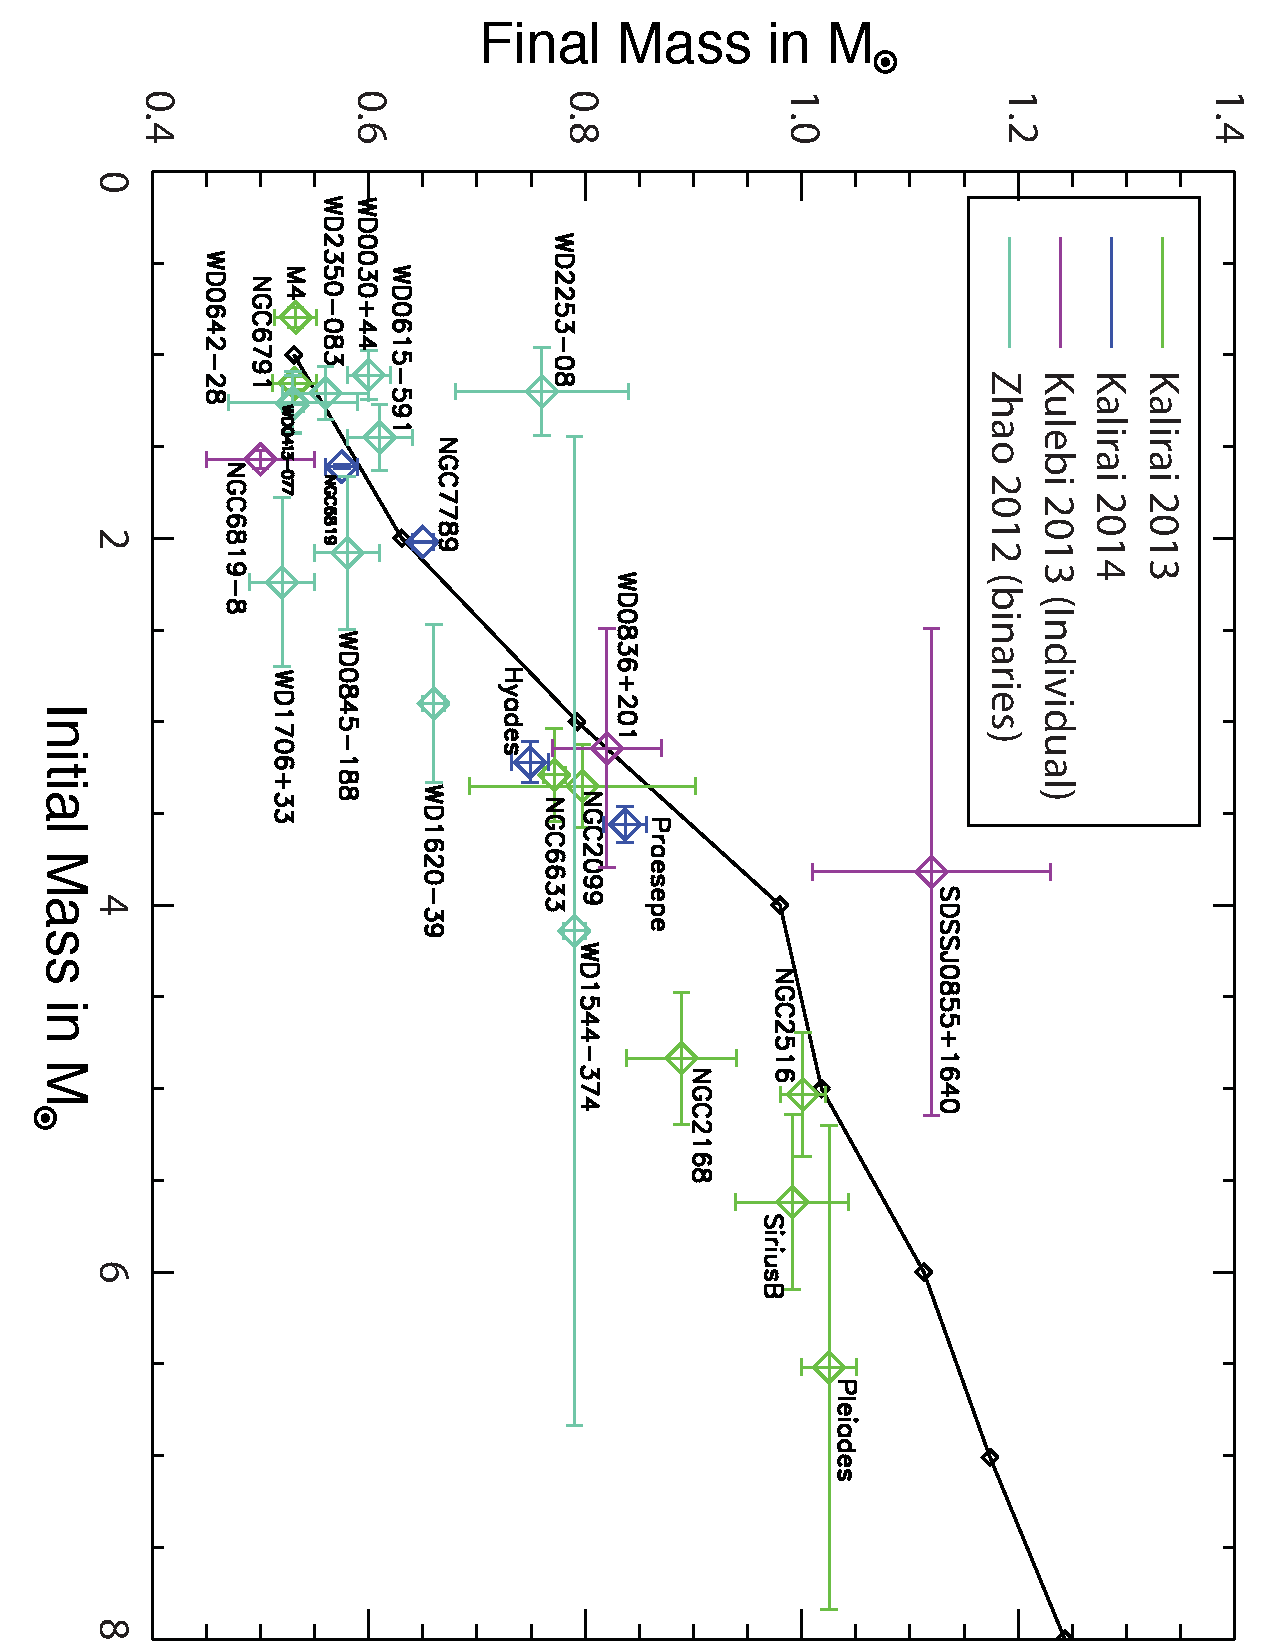
\includegraphics[width=0.35\textwidth, angle=90]{if_mod2.pdf}
\caption{ Initial final mass relation from observations and MESA calculations. The \citealt{kalirai2013a} and \citealt{kalirai2013b} points are averaged over the total observed white dwarfs in each respective cluster, while the \citealt{kulebi2013} and \citealt{zhao2012} points are taken from individual observations.}
\label{fig:ifrelation}
\end{figure} 

\begin{figure}
\centering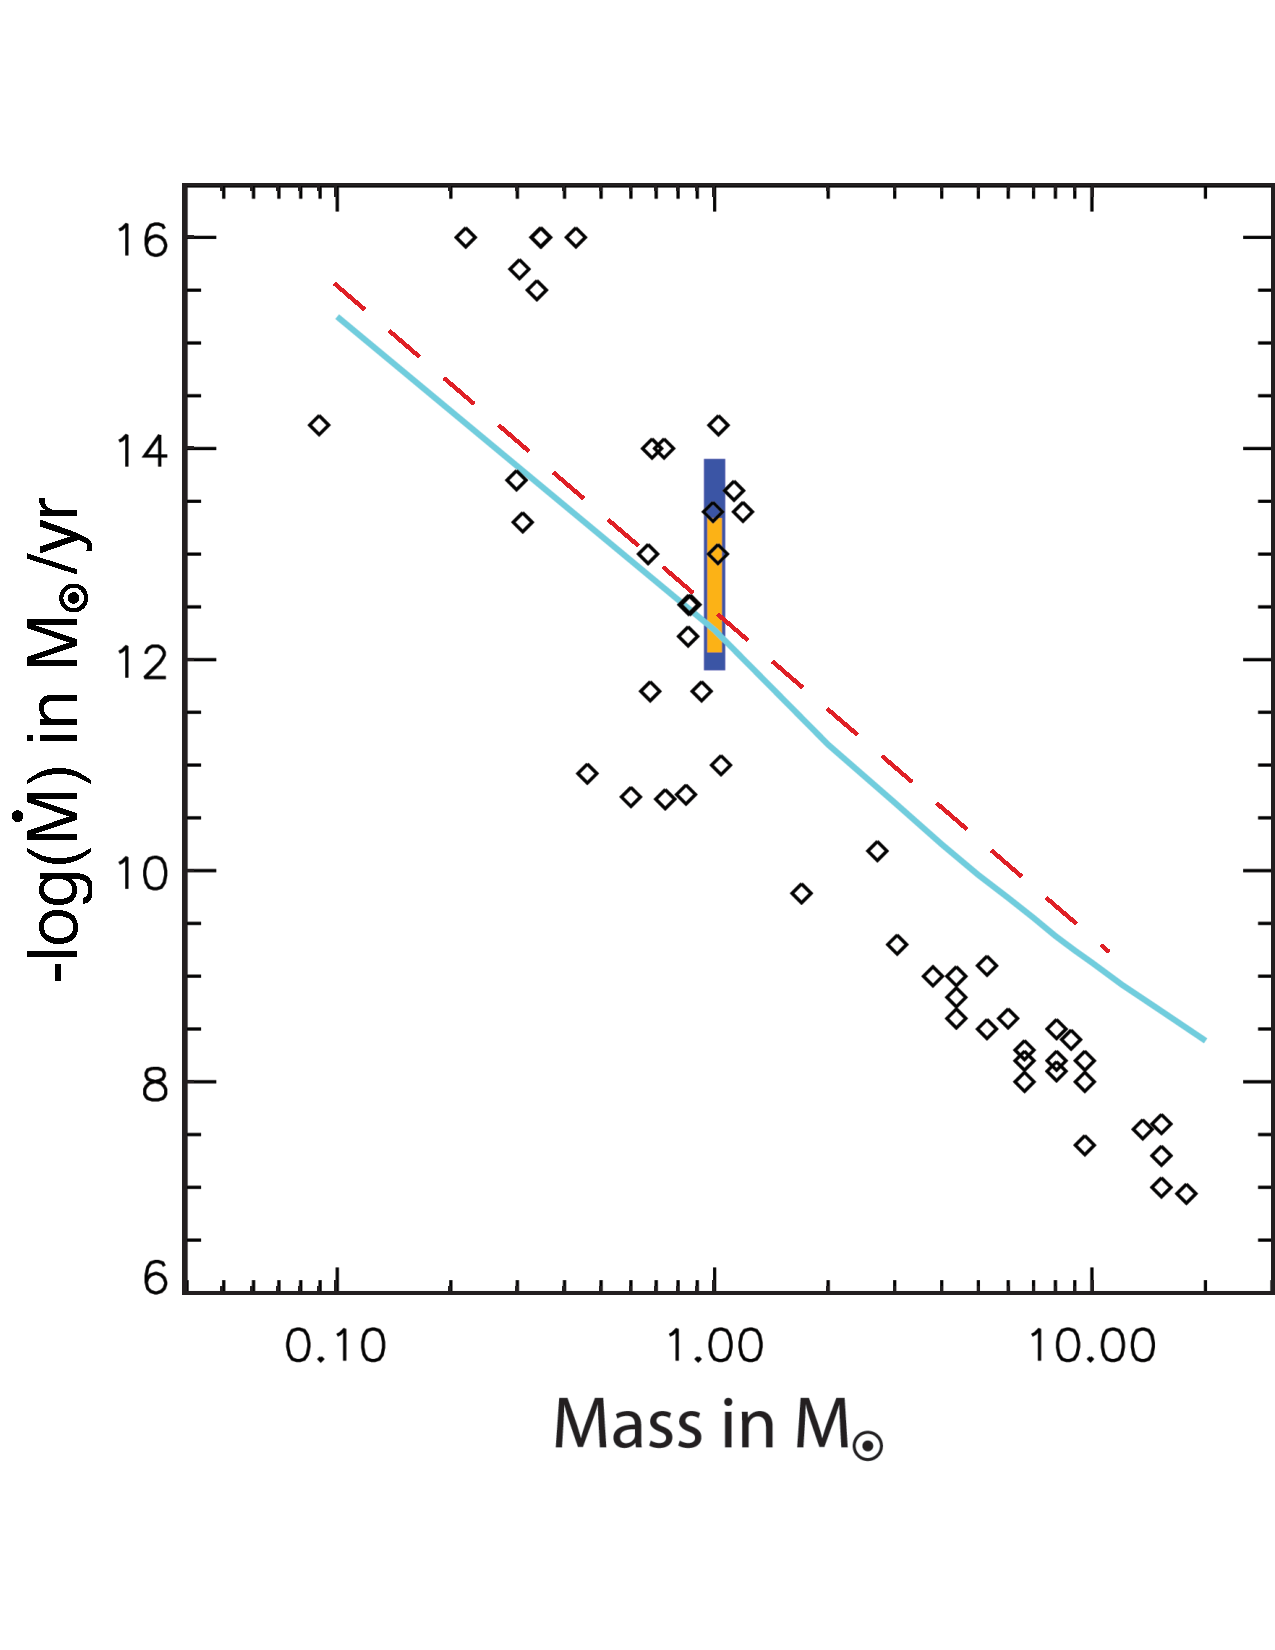
\includegraphics[width=0.46\textwidth]{mdotms_withAnalytic_mod3.pdf}
\caption{Mass loss rate estimates along the main sequence as a function of initial stellar mass.  Observational estimates are plotted as black diamonds \citep{cranmer2011,dejager1988,searle2008,waters1987,debes2006,badalyan1992,morin2008}.  The blue rectangle denotes the estimated variations in the solar mass loss rate \citep{wood2005}, and the yellow rectangle shows the observed variations in the mass loss rate of the Sun as a function of its X-ray activity \citep{cohen2011}.  The blue line shows the main sequence mass loss rate prescription used by MESA and the often derived analytical prescription is shown with the dashed red line. }
\label{fig:msmassloss}
\end{figure} 


\subsubsection{Wind Velocities}


Shortening here as well.

\subsection{Average Mass Loss and Wind Velocities as Model Inputs} \label{section:averages}

To finalize our mass and energy injection prescriptions it is necessary to derive an averaged mass loss rate and wind velocity during each phase of cluster evolution which includes contributions from the stars that significantly contribute to the mass and kinetic energy injection into the cluster.
The averaged prescription we present here has the added benefit of minimizing the effects of the poorly constrained, rapidly varying, final stages of a star's life \citep{pooley2006}.


Note: more shortening is happening here too.

\section{Applications to Various Star Clusters} \label{section:applications}

We have thus far kept our discussion of stellar wind retention in star clusters generalized to star clusters with different combinations of ages, masses and velocity dispersions.  In what follows we discuss the implications of gas retention on three specific groups of star clusters - Young Massive Clusters, Intermediate Age Clusters, and Globular Clusters - and provide limits on how stellar wind retention can effect their star formation histories.


\subsection{Young Massive Clusters: Age $\lesssim$1~Gyr}

Young, massive star clusters (YMCs) are ubiquitous in the nearby Small and Large Magellanic Clouds \citep{goud2014} and are also found in recent ($\lesssim$1~Gyr) mergers like the Antennae galaxies \citep{whitmore2007}.  As one of the canditates for proto-Globular Clusters, the gas content and star formation histories of these objects are a subject of much interest \citep[e.g.][]{zwart2010}.

\subsubsection{Current Gas Content} \label{section:YMCcurrent}

 During the time span of the typical ages of YMCs (10s-100s~Myrs) Figures \ref{fig:fig4} - \ref{fig:memcontour} show little mass retention and star formation in all but the most compact stellar clusters.
 This results from the fast winds from main sequence O and B stars as shown in Figure \ref{fig:fig1} for ages $\lesssim 20$~Myrs, and the lack of sufficient gas accumulation time to initiate runaway cooling and collapse for clusters with $20 \lesssim {\rm age/Myrs} \lesssim 500$.
 For clusters with large velocity dispersions, $\sigma_v \gtrsim 35 \, {\rm km s^{-1}}$, while some gas mass is retained and star formation is triggered, less than $\approx 2$\% of the original cluster's mass is available for star formation.

 In such clusters we expect several additional mechanisms to add significantly to the energy injection rate in the intercluster gas.
 As shown in \cite{calura2015} SNe can be an effective avenue to assist in the removal of gas from stellar clusters, though in some systems SNe alone may not be able to fully remove gas from young clusters \citep{krause2013}.
 In addition, accretion onto compact objects may be able to clear gas within YMCs on time scales as small as 10~Myrs \citep{leigh2013a}.
 Finally, Lyman-Werner flux from massive stars further inhibits star formation by dissassociating molecular hydrogen in these young systems \citep{ten1986,conroy2011b,krause2013}.
 Therefore, we conclude that our estimates of gas retention on the order of a few percent are upper limits for the total mass retained from stellar wind ejecta within YMCs.

 Such a small amount of gas retention is broadly consistent with both observations and more complex simulations.
 Recent observations which show little gas in all but the most compact clusters \citep{bastian2014a,cabrera2015,krui2015,longmore2015}, though observations at high redshift are challenging \citep{longmore2015}.
 Our results are also consistent with analytic and three dimensional simulations of  which find that the majority of gas mass is removed by $1-14$~Myrs \citep{calura2015,krui2015}.


\subsubsection{Previous and Ongoing Star Formation} \label{section:YMCongoing}

 Our results of little to no star formation in Figures \ref{fig:fig4} - \ref{fig:memcontour} over the several hundreds of Myrs timespan are broadly consistent with the results of \cite{bastian2013a} which show no ongoing star formation in 130 YMCs with masses ranging from $10^4 < M/M_\odot < 10^8$ and ages $10 < {\rm age/Myrs} < 1000$ and \cite{mart2018} who only find MSPs in clusters with ages $\gtrsim 2$~Gyr, though our level of predicted star formation may be too low to be detectable in the majority of YMCs \citep{peacock2013}.
  Our limit of $\sigma_v \gtrsim 35 \, {\rm km s^{-1}}$ is a slightly higher limit for velocity dispersion than that derived observationally from assuming eMSTO features in IACs \citep{goud2014} are due to an age spread.  Such a discrepancy can be alleviated if assumed evolution of the velocity dispersion changes more dramatically from YMC to IAC stage than assumed in \cite{goud2014} or if the eMSTO feature is due to a population of rapidly rotating main sequence stars  \citep{cabrera2016,bastian2016,piatti2016} or other stellar evolutionary affects \citep{bastian2017}.
While \cite{li2016} see evidence for past star formation in IACs which are less massive and more diffuse clusters than predicted by our simulations, their suggestion that these episodes of star formation may have been triggered by the accumulation of gas from the clusters as they orbited within the gaseous disk of their host galaxy is not necessarily inconsistent with this work as we assume our stellar wind material is accumulated in star clusters in isolation.  Previous work has shown that cold gas accretion may indeed be a viable avenue for significant gas retention and star formation \citep{naiman2009,conroy2011a,conroy2011b,priestley2011,naiman2011,conroy2012}, however our detailed treatment of the interplay between these two gas accumulation processes is left to a subsequent paper. 


Continuing to shorten here.





\section{Summary and Conclusions} \label{section:conclusions}

 We have presented a grid of spherically symmetric simulations of gas retention and expulsion due to stellar winds within star clusters.
 While previous work has estimated the ability of star clusters to retain stellar winds \citep{dercole2008,dercole2010,vesperini2010,conroy2011b,conroy2011a}, calculations have so far been under taken over a smaller range of cluster properties and stellar ages, typically with lower stellar wind velocities than those argued for in this work.
 Motivated by this, we have calculated gas retention in  star clusters of various ages, stellar mass and compactness.  
 Additionally, we include a discussion of the choice of the kinetic energy injection proxy, taken here as the wind velocity, $v_w$, and its relation to the observed distribution of outflow velocities observed in field and globular cluster AGB and RGB stars.  \\
 \\
\noindent Our main conclusions are the following:

\begin{easylist}[itemize]

& We conclude that in compact star clusters a choice of $v_w = v_{\rm esc}$ best reproduces both the observations of stellar winds and the assumed level of mixing between stellar wind and the intercluster medium.

& Given our assumptions about the mass loss rates and wind velocities emanating from stars residing in clusters, we find the optimum time for gas retention is approximately 1-2~Gyrs.  However, depending on how efficiently the slow winds from AGB/RGB stars mix with the fast winds from the numerous main sequence cluster members, and how effectively gas is cleared after each episode of star formation within the cluster, we find star formation may not be triggered within this optimum time span as the gas may be too hot.

& We find significant gas retention can occur when cluster velocity dispersions are high, $\sigma_{\rm v} \gtrsim 25 \, {\rm km s^{-1}}$, but the amount of gas retained drops as the velocity dispersion grows due to the efficient funneling of gas to the central regions of the cluster and subsequent triggering of star formation for very compact clusters.

& We compare our results with observations of young massive clusters (YMCs), intermediate age clusters (IACs) and globular clusters (GCs).  We find our models generally agree with observations.  We predict little gas retention and star formation in YMCs and GCs.  Our models predict higher levels of gas retention in IACs ($\approx 10\%$ of the stellar mass).  However, we caution that both the lack of observations of isolated IAC systems and the lack of inclusion of all the sources of thermal and kinetic energy in star clusters in this age range makes any conclusions drawn from our models preliminary.  

& Finally, we discuss the implications of our models on the assumed evolutionary sequence of YMC$\rightarrow$IAC$\rightarrow$GC resulting in observations of multiple sub-populations with different levels of light element enhancement in present-day GCs.  The majority of proposed origins for these sub-populations rely on some amount of gas retention in the age range few-100s of Myrs. However, we find hot stellar winds are effective at driving material from the cluster during this time frame for all but the most massive and compact clusters.  This result is problematic for the AGB wind retention scenario \citep{dercole2008,dercole2010,conroy2011a,conroy2011b} invoked to explain the abundance anomalies observed in present day Galactic globular clusters, but if hot stellar winds can effectively thermalize with the intercluster medium during this time, our models pose problems for gas retention in the early disk accretion \citep{bastian2013a} and fast rotating massive stars \citep{krause2013} scenarios as well.

\end{easylist}

$\,$\\

\noindent In this work, we have also tried to minimize the effect of external mass inflow by considering star clusters in isolation. This is certainly not the case for clusters moving through cold, dense environments, as they  can potentially 
amass a significant amount of gas from their surroundings \citep{naiman2009,naiman2011}, or clusters moving quickly though hot halo gas or the galactic disk \citep{priestley2011}.  If the star clusters reside  within cold gas, stellar winds and exterior inflows in such clusters could combine 
to create even larger central density enhancements \citep{naiman2009,pflamm2009,naiman2011,conroy2011a}.  
Additionally, one dimensional spherically symmetric models cannot accurately model all multi-dimensional phenomena. For example, these simulations are not able to follow the effects of cool fragments which may exist in otherwise hot gas, thereby overestimating the effects of hot gas expelling material from the cluster \citep{krause2012}.
A  self consistent  treatment  of both interior and exterior gas  accumulation in multi-dimensional simulations,  which includes the effects of compact object accretion, tidal stripping, photoionization, and pulsar heating will be presented elsewhere. 






%-------------------------------------------------------------------------------------------------



\section*{Acknowledgements}

We thank Mark Krumholz, Charlie Conroy, David Pooley, Rebecca Bernstein, Chung-Pei Ma and Morgan Macleod for useful discussions, and we thank the referee for their helpful comments. The software used in this work was in part developed by the DOE-supported ASCI/Alliance Center for Astrophysical Thermonuclear Flashes at the University of Chicago. Computations were performed on the Pleaides/Hyades UCSC computer cluster. This work is supported by NSF: AST-0847563, NASA: NNX08AL41G, NSF AARF award AST-1402480, and The David and Lucile Packard Foundation.


\bsp	% typesetting comment



%%%%%%%%%%%%%%%%%%%%%%%%%%%%%%%%%%%%%%%%%%%%%%%%%%

%%%%%%%%%%%%%%%%%%%% REFERENCES %%%%%%%%%%%%%%%%%%

% The best way to enter references is to use BibTeX:

%\bibliographystyle{mnras}
%\bibliography{example} % if your bibtex file is called example.bib




\bibliographystyle{mnras}

\bibliography{bib_agb_2016}




%%%%%%%%%%%%%%%%%%%%%%%%%%%%%%%%%%%%%%%%%%%%%%%%%\
% Don't change these lines
%\bsp	% typesetting comment
%\label{lastpage}
%\end{document}

\label{lastpage}
\end{document}


